\chapter{xSort}

\label{chap:tool}

xSort is an offline card sorting tool which only provides a local version for 
macOS. In contrast to other modern tools it is not up to modern standards. 
Both the design and the handling are no longer up to date, as you can 
see in Figure~\ref{fig:xSort-sorting}. Because of being free of charge it is 
still an alternative for local card sorting on macOS. Furthermore also the 
few existing analysis tools can be used completely free of 
charge~\parencite{xSort}.



\begin{figure}[tp] 
\centering
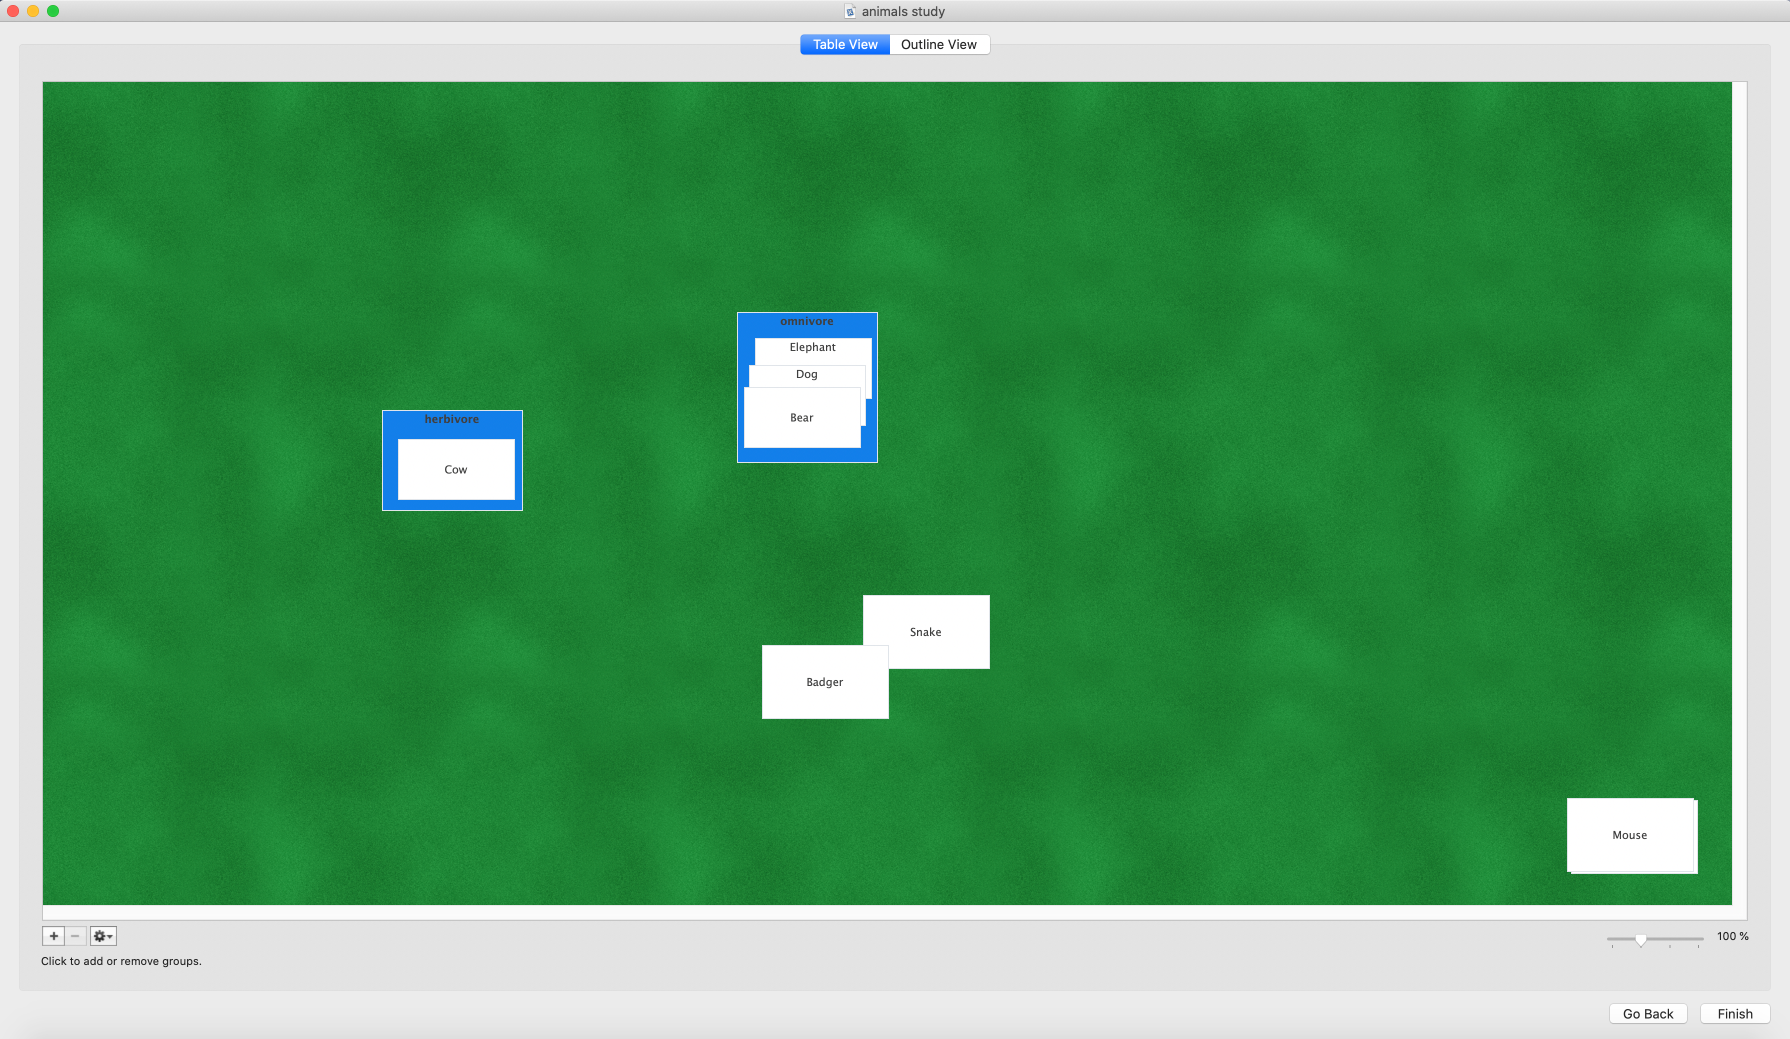
\includegraphics[keepaspectratio,width=\linewidth,height=\halfh]{images/xsort-sorting.png}
\caption[xSort Application] { This screenshot shows the sorting in the table view of xSort.
\imgcredit{Screenshot was captured by Markus Stradner using
\textcite{xSort} on macOS Catalina 10.15.7, 28.11.2020.} }
\label{fig:xSort-sorting}
\end{figure}



\section{Business Model}

The tool is fully free of charge, so no features are hidden behind a 
paywall. It was created by the Enough Pepper company and is 
currently not maintained. As it is a local program you don't need 
to create an account.



\section{Card Sorting}

The setup process of a card sorting is quite simple and works well. As 
you can see in Figure~\ref{fig:xSort-setup}, all the settings can be 
made on one site. You can also type in welcome and thank you 
messages. The cards and categories (for closed card sorting) can be 
imported via .csv file. Also names for different user profiles can be 
set.



\begin{figure}[tp] 
\centering
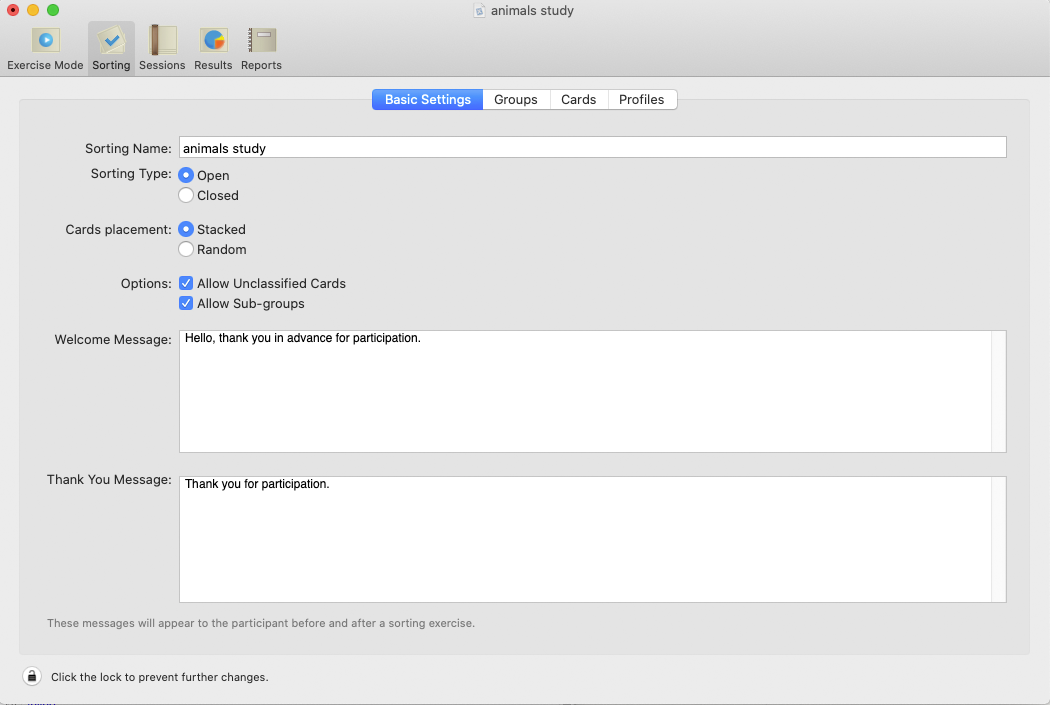
\includegraphics[keepaspectratio,width=460px]{images/xsort-setup.png}
\caption[xSort Setup] { This screenshot shows the setup view of xSort.
\imgcredit{Screenshot was captured by Markus Stradner using
\textcite{xSort} on macOS Catalina 10.15.7, 28.11.2020.} }
\label{fig:xSort-setup}
\end{figure}



In the exercise mode which is the mode to run through the study 
you have to select your profile, your gender and have to type 
in your age. After that you can change between the table view 
and an outline view during the whole sorting. In the table view 
you have to pick up the cards in the bottom right corner and 
assign it to the desired group. If you would like to use the 
outline view you have to drag the card items on the left side 
to the desired group item on the right side. 

At an open card sorting you have to create the categories yourself, 
which is also not so convenient. Because there is no 
auto-alignment of the groups and the cards, the clean up 
tool exists to align all the elements on a grid via the gearwheel 
button where you can also restart the card sorting. 

xSort also offers a zooming tool to zoom in and out
of the grouping area. But this is not very practical, because 
you have troubles with scrolling and seeing all the elements 
if you zoom in. 

One feature no other tool has is that it is possible to group in 
sub-categories. This is allowed in both the table view and the 
outline view. Sometimes errors occur during sorting. Then 
no more cards can be moved. This occurs especially in the 
outline view, which is shown in Figure~\ref{fig:xSort-outlineview}.



\begin{figure}[tp] 
\centering
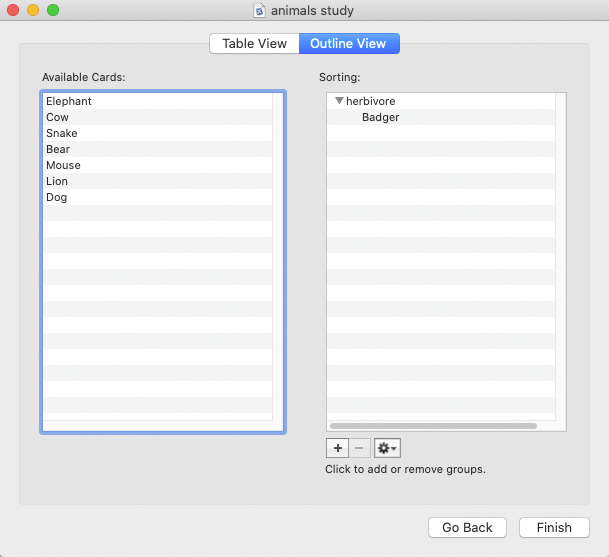
\includegraphics[keepaspectratio,width=460px]{images/xsort-outlineview.png}
\caption[xSort Outline View] { This screenshot shows the outline view of xSort.
\imgcredit{Screenshot was captured by Markus Stradner using
\textcite{xSort} on macOS Catalina 10.15.7, 28.11.2020.} }
\label{fig:xSort-outlineview}
\end{figure}



\section{Analytics}

The tool also includes a few analysis tools. But the extent of 
these is not comparable to that of OptimalSort for example. 
It just offers a cluster tree, general statistics like unclassified 
cards, number and average duration of the participations 
and a distance table.  

With xSort, however, the age, gender and profile can also 
be taken into account in the evaluation. You can filter the 
results by those user attributes and create a report accordingly, 
which you can then save as a PDF or print directly. But also 
in that area the design is very bad and except the cluster 
tree no graphics are displayed, as you can see in
Figure~\ref{fig:xSort-cluster}.

For generation of such a report you have to choose the 
desired components. You can select the following ones: 
Problem Information, cards, groups, profiles, sessions, 
unclassified cards, cluster tree, marks. If you would like 
to generate a cluster tree you can select a single linkage, 
average linkage or complete linkage and you can also 
differ to flatten groups or use sub groups.



\begin{figure}[tp] 
\centering
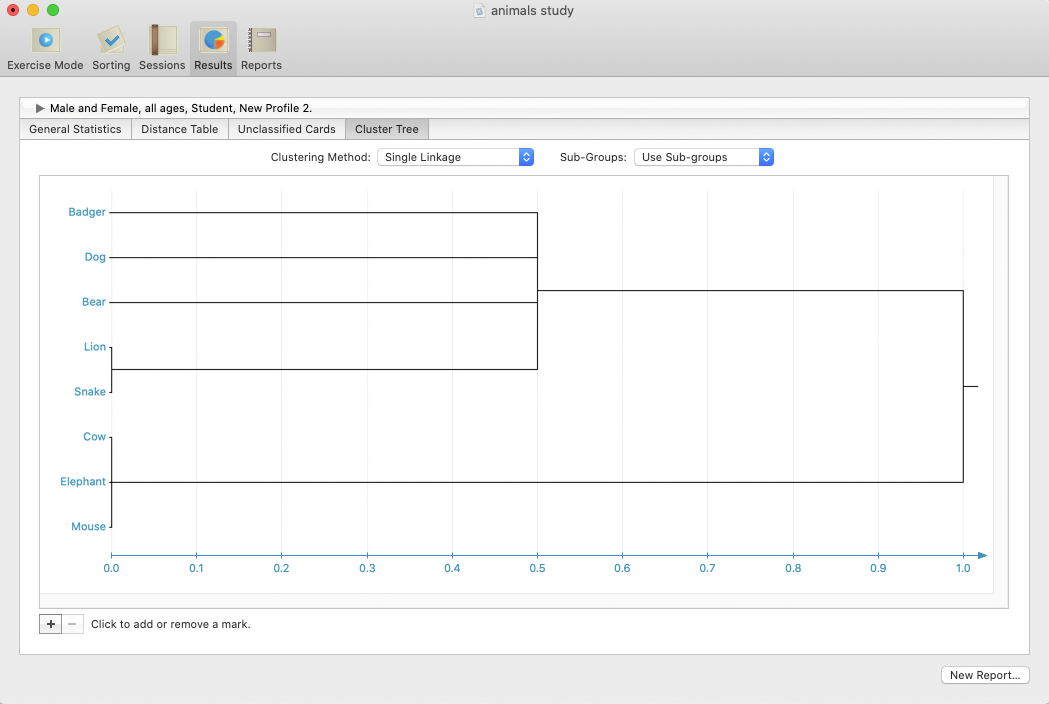
\includegraphics[keepaspectratio,width=460px]{images/xsort-analysis.png}
\caption[xSort Analysis] { This screenshot shows a cluster tree in the results section of xSort.
\imgcredit{Screenshot was captured by Markus Stradner using
\textcite{xSort} on macOS Catalina 10.15.7, 28.11.2020.} }
\label{fig:xSort-cluster}
\end{figure}



\section{Summary \& Ratings}

In comparison with more modern card sorting tools like 
OptimalSort, in xSort there is a password security possible, 
it has a zooming tool, a clean up tool and the biggest advantage 
is, that it’s free of charge.

The main disadvantages are that it can’t be used for online 
studies, the design is very bad and not up to date, there are 
also small bugs in it. The documentation stuff can only be found 
online and while assigning the cards, the groups don’t align 
with the grid. So there is a mess after assigning more cards 
and you have to use the clean up tool very often. A detailed 
summary of features can be viewed in
Table~\ref{tab:features-xSort}. 

\begin{table}[tp]
\centering
\begin{tabularx}
{\linewidth}{|l|X|}
\hline \textbf{Feature/Characteristic} & \textbf{Availability in xSort} \\ 
\hline Card Sorting & Open and closed. \\ 
\hline Card Limit & No. \\
\hline Participant Limit & No. \\
\hline Analytics & Cluster tree, general statistics and distance table. \\ 
\hline Documentation & Instructions can be found online. \\
\hline Business Model & Fully free of charge. \\
\hline Import formats & .xml, .csv \\ 
\hline Export formats & .xml, .csv, .html, .pdf \\ 
\hline Sub-Categories & Yes. \\ 
\hline Playback of user-sessions & No. \\ 
\hline Data preparation & Only by hand through export reports. \\ 
\hline
\end{tabularx} 
\caption[Feature summary of xSort] 
{ 
This table summarizes all the features and characteristics of xSort
to provide an easy to read overview.
}
\label{tab:features-xSort}
\end{table}



The ratings for the tools can be found in a short overview in
Table~\ref{tab:rating-xSort} and range from 0-5.



\begin{table}[tp] 
\centering 
\begin{tabularx}{\linewidth}{|X|X|X|X|X|}
\hline
Simplicity & Documentation & Features & Business Model & Average \\ 
\hline 
2 & 2 & 3 & 4 & 2.75 \\ 
\hline 
\end{tabularx} 
\caption[Ratings for xSort] {
Ratings for xSort including the average rating.
} 
\label{tab:rating-xSort}
\end{table}
